%!TEX root = ../thesis.tex
%*******************************************************************************
%*********************************** Fourth Chapter *****************************
%*******************************************************************************

\chapter{Discussion}  %Title 

\ifpdf
    \graphicspath{{Chapters/Chapter5/Figs/Raster/}{Chapters/Chapter5/Figs/PDF/}{Chapters/Chapter5/Figs/}}
\else
    \graphicspath{{Chapters/Chapter5/Figs/Vector/}{Chapters/Chapter5/Figs/}}
\fi


%********************************** %First Section  **************************************
\section{How to improve Gaps to Trips?}

The initial idea for this work was to identify foragers using just statistical inference, without supervision from a labeled dataset. This was in hope that the 
signal would be clear enough that basic knowledge of what to expect from a forager's behaviour
would be enough to interpret it. If I saw clear spikes in amount of trips taken, among bees that are in the right age groups, that would be the case.

Instead, because of the extreme amount of noise I found when trying to find Trips among Gaps, I ended up manually labeling videos to make sure my outputs are still grounded in truth. This is unfortunate, 
as the labor of manual observation is exactly what the BeesBook project is trying to spare - but it did spark the idea to manually label enough examples to be able to train a classifier. While the required effort could prove to be quite high, it is important to note that it would only need to be made once. It's a path I did not pursue further, as the amount of work it would require was outside the scope of this project. I do, however, discuss how I would go about it in the Future Work section. %TODO

\section{Parameter tuning}

One of the main reasons I was longing for a labeled dataset was adjusting hyperparameters. The model I created for reasoning about foragers is, in the end, very simple - and yet it unavoidably depends on a few hyperparameters, creating a large number of possble combinations for their values. Most of those I needed to choose half-intuitively, after some experimenatation, as properly testing any one was not really possible without a labeled dataset. This created some degree of uncertainty in the latter stages of the process. While my choices were (to some extent) validated by both Presence and Gaps showing consistency with manual video observation, it would have been much more comfortable to be able to set up a testing framework for them.


\begin{figure}[htbp!] 
\centering    
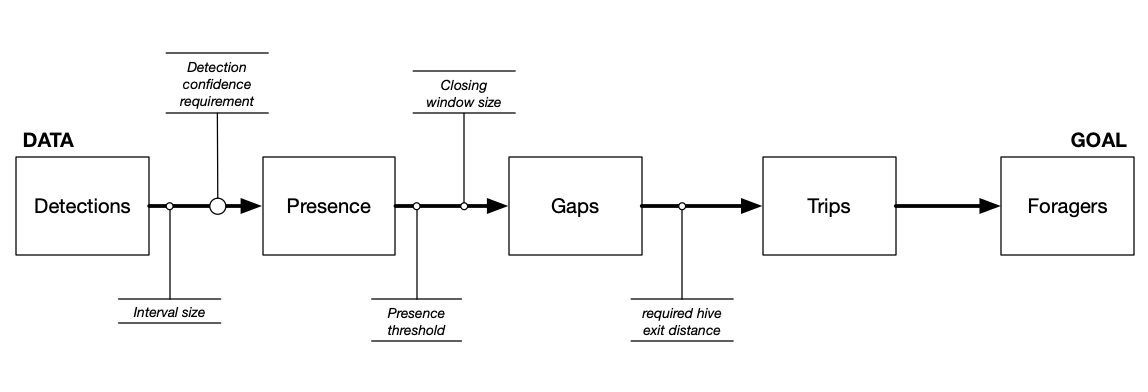
\includegraphics[width=1.0\textwidth]{funnel-params}
\caption[funnel-params]{Visualization of the abstraction steps, with some of the parameters involved in creating them. Emphasized is the only parameter that has been reliably tested for a better value}
\label{fig:funnel-params}
\end{figure}




\section{Contributing abstractions}

While unsuccessful in detecting forager transitions, I'm contributing the concepts of Presence and Gaps, along with the code for computing them and the idea of generating those concepts often and saving well. I hope that will genuinely have a positive influence on future investigations, perhaps also involving the foraging question.

